\documentclass{pracamgr}  
\usepackage{lmodern} 
\usepackage[polish]{babel} 
\selectlanguage{polish} 
\usepackage{fontspec}
\usepackage{minted}
\usepackage{listings}
% package for hyperinks
\usepackage{hyperref}
\usepackage{amsmath, amsthm, amssymb}
\usepackage[ansinew]{inputenc}
\usepackage{svg}
\usepackage{eucal}
\usepackage[mathcal]{eucal}
\usepackage[mathscr]{eucal}
\hypersetup{
    colorlinks,
    citecolor=black,
    filecolor=black,
    linkcolor=black,
    urlcolor=black
}
\usepackage{graphicx}  
\usepackage{makeidx}
\makeindex
\linespread{1.5} 
 

\makeatletter
\def\l@lstlisting#1#2{\@dottedtocline{1}{1.5em}{3em}{#1}{#2}}
\makeatother


\definecolor{grey}{gray}{0.9}
\definecolor{bg}{HTML}{FAFAFA}
\definecolor{darkgray}{HTML}{D5D5D5} 
% \newgeometry{left=25mm,right=0.8in,top=25mm,bottom=25cm}

% \renewcommand\lstlistlistingname{}
\renewcommand*{\listlistingname}{Lista kodów źródłowych}
\makeatletter
\raggedbottom
% \renewcommand{\lstlistlistingname}{Spis kodów źródłowych}
\renewenvironment{minted@colorbg}[1]{
\linespread{1.0} 
\setlength{\fboxsep}{\z@}
\def\minted@bgcol{#1}
\noindent
\begin{lrbox}{\minted@bgbox}
\begin{minipage}{\linewidth}}
{\end{minipage}
\end{lrbox}%
\colorbox{\minted@bgcol}{\usebox{\minted@bgbox}}}
\makeatother

%Jesli uzywasz kodowania polskich znakow ISO-8859-2 nastepna linia powinna byc odkomentowana
%Jesli uzywasz kodowania polskich znakow CP-1250 to ta linia powinna byc 
%odkomentowana
%\usepackage[cp1250]{inputenc}

% Dane magistranta:

\author{Konrad Lisiecki}
\nralbumu{48211}
\title{Wycena Opcji przy pomocy Modeli Zmienności Stochastycznej} 
\kierunek{Finanse i rachunkowość}
\instytut{Ekonometrii}
\opiekun{dra hab. Łukasza Delonga} 
\date{Warszawa 2015}   
% Tu jest dobre miejsce na Twoje własne makra i~środowiska:
\newtheorem{defi}{Definicja}[section]
\newtheorem{prop}{Własność}

% koniec definicji 

 


%===========================================================================
%                             Bibliogrphy
%=========================================================================== 
\usepackage[style=numeric,sorting=ydnt,defernumbers=true, backend=bibtex]{biblatex}
\addbibresource{biblio.bib}
 
%===========================================================================
%                               Listings
%===========================================================================
\renewcommand\listoflistingscaption{Spis kodów źródłowych}
\renewcommand\listingscaption{Kod źródłowy}

\usepackage{chngcntr}% http://ctan.org/pkg/chngcntr
\counterwithin{listing}{chapter}

%===========================================================================
%                           Begin of document 
%===========================================================================


\begin{document}
\maketitle
\nocite{book-full} 

%===========================================================================
%                               Introduction
%===========================================================================
\chapter*{Streszczenie} 


Tematem pracy magisterskiej jest wycena opcji przy pomocy modeli zmienności stochastycznej. 
W standardowych modelach służących do wyceny opcji przyjmuje się (jak np. w modelu 
Blacka-Scholesa), że zmienność jest wartością stałą, niezależną od czasu. 
Jednak jak dalekie jest to założenie od rzeczywistości pokazał chociażby ostatni kryzys 
ekonomiczny, gdzie kursy instrumentów finansowych wahały się o wiele bardziej niż w czasach
koniunktury gospodarczej. W bardziej ogólnych modelach służących do wyceny opcji uziemienia się parametr opisujący zmienność instrumentów finansowych i uzależnia się go od czasu. 


Po wstępie, w drugim rozdziale zostanie przedstawiony schemat budowania symulacji w oparciu o metodę Monte Carlo. Będzie się to odbywało na przykładzie wyceny opcji w modelu Blacka-Scholesa, który 
jest jednym z najprostszych modeli do wyceny opcji.

W trzecim rozdziale zostanie opisany model Hestona i sposób w jaki można wyliczyć. 
Zostaną przedstawione kroki jakie należy poczynić, aby wycenić opcję przy pomocy tego modelu.

Czwarty rozdział z kolei jest poświęcony kalibracji modelu, czyli inaczej ujmując, znalezieniu 
optymalnych wartości nieznanych parametrów modelu. Optymalna wartość jest w tym przypadku zdefiniowana
jako taka, dla której wartość opcji, wyliczonej na podstawie modelu Hestona, jest najbliższa wartości 
obserwowanej na rynku.

W przedostatnim rozdziale zostaną przedstawione możliwości dalszych uogólnień modelu Hestona. 
Polegają one głównie na próbie uzmiennienia (uzależnienia od czasu) tych wartości parametrów, które w 
modelu Hestona są stałe w czasie.

Ostatni rozdział to już próba empirycznego zbadania zachowania modelu Hestona. Zostanie w nim porównana
wartość opcji na indeks \textit{S\&P500} stosując odpowiednio model Blacka-Scholesa i model Hestona.



%===========================================================================
%                               Table of contents
%===========================================================================
\tableofcontents


%===========================================================================
%                               Wprowadzenie
%===========================================================================
\chapter{Wprowadzenie}
\label{chap:introduction}
\begin{quote}

  We developed what is known a stochastic volatility model. 
  This is a model where the volatility as well as the 
  underlying asset price moves around in an unpredictable way.

\raggedleft\slshape John Hull \index{Hull, John}
\end{quote}
Niniejsza praca jest poświęcona modelom zmienności stochastycznej używanych przy wycenie opcji. 
Nasuwa się jednak pytanie, czym dokładnie są te modele? 
Jaka jest ich istota? Jaka motywacja stoi za ich powstaniem?


Bardzo zwięzłej, a zarazem trafnej odpowiedzi na te pytania udziela John Hull, 
jeden z pionierów dzisiejszych finansów ilościowych. Stwierdza on, zgodnie z przytoczonym 
powyżej cytatem, że są to modele, gdzie nie tylko cena aktywa bazowego, ale również jego zmienność, 
poruszają się w sposób nieprzewidywalny, losowy. 

W niniejszej pracy przedstawiony zostanie model Hestona, w którym zmienność nie jest wartością stałą 
oraz sposób wyliczenia wartości opcji przy pomocy tego modelu.
Część empiryczna pracy jest z kolei próbą sprawdzenia, jak model, oraz narzędzia do jego stosowania, sprawdzają się w praktyce.

W dalszej części tego rozdziału, zostaną przedstawione motywacje rozwoju takich modeli oraz w jaki sposób
wpływają one na dokładność analizy finansowej i efektywność rynków finansowych. 


\section{Rys historyczny} % (fold)
\label{sec:rys_historyczny}

Do lat '90 XX wieku podstawowym modelem do wyceny opcji był model Blacka-Scholesa. Opublikowany w 1973 \cite{BlackScholes} roku artykuł, którego autorami byli \textbf{Fischer Black} oraz \textbf{Myron Scholes}, był przełomowy dla teorii wyceny opcji.
U jego podstaw leży bardzo istotne założenie mówiące o tym, że zmienność instrumentów finansowych jest stała w czasie. 
Niestety, założenie to jest niezgodne z tym, co możemy obserwować na rynkach finansowych. 
Można to szczególnie mocno zauważyć w czasie cyklicznie powtarzających się kryzysów finansowych.

Obserwowalna duża zmienność w czasie parametru zmienności na rynkach finansowych stała się podstawową motywacją wprowadzenia modeli wyceny
opcji, dla których zmienność nie jest ustalonym parametrem, a zmienną zależną od pewnych innych czynników. 
Pionierem w tym obszarze okazał się \textbf{Steven Heston}\index{Heston, Steven}, który w 1993 opublikował pracę, gdzie wprowadza
nowy model wyceny opcji, w którym nie tylko proces cen instrumentu bazowego, ale również
proces zmienności jest stochastyczny (losowy) i zależny od czasu \cite{Heston}. Na jego cześć, model ten 
w literaturze znany jest pod nazwą modelu Hestona.
 

\section{Wycena opcji na potrzeby rynków finansowych} % (fold)

Instrumenty pochodne, a w szczególności opcje, są dzisiaj bardzo ważną klasą instrumentów finansowych i stanowią znaczną 
część wartości obrotu na światowych giełdach.

Światowy rynek derywatów, który dziś jest warty około 450 mld EUR \cite{GlobalDerMarket}, jeszcze około 25 lat temu był bardzo mały. Powstaje więc pytanie co wpłynęło na rozwój tego typu transakcji na globalnym rynku? Z punktu widzenia rynku finansowego jest jedno wytłumaczenie tego zjawiska:
instrumenty pochodne, a szczególnie opcje, pozwalają na handel przyszłym ryzykiem związanym z ruchem cen instrumentów bazowych. W związku z tym można wyróżnić dwa podstawowe 
zastosowania opcji: 

\begin{enumerate}
  \item jako element zarządzania ryzykiem (\textit{ang. hedging})
  \item jako inwestycja 
\end{enumerate}

Pierwsze zastosowanie odnosi się do wymiany lub ograniczenia ryzyka rynkowego. Przedsiębiorstwa i instytucje finansowe używają opcji do 
ochrony przed niechcianymi, gwałtownymi ruchami instrumentów bazowych takich jak surowce, stopy procentowe czy kursy akcji. Wpływa to na 
\textbf{wygładzenie przepływów pieniężnych} (\textit{ang. cash flows}} w obrębie przedsiębiorstwa, co wpływa na stabilność działalności 
podmiotu gospodarczego. Dla przykładu, 92\% spośród 500 największych przedsiębiorstw świata ogranicza ryzyko przy pomocy derywatów \cite{GlobalDerMarket}.


Transakcje na runku instrumentów pochodnych są szczególnie ważne z punktu widzenia ograniczenia \textbf{ryzyka walutowego}. Na rysunku \ref{fig:currencyRisk} przedstawiono kurs dolara amerykańskiego w stosunku do rosyjskiego rubla na przestrzeni ostatnich 20 lat.

\begin{figure}
  \centering  
  \includegraphics[width=0.80\textwidth]{../figures/currencyUSDRUB.pdf}
  \caption{Kurs walutowy rosyjskiego Rubla w stosunku do Dolara amerykańskiego.}\label{fig:currencyRisk}
\end{figure} 
Można na nim odnotować gwałtowne wahania kursu, które dla wielu przedsiębiorstw, nie stosujących instrumentów pochodnych w celu ograniczenia ryzyka walutowego, może oznaczać bardzo szybkie bankructwo. 
 
Instrumenty pochodne mogą być również postrzegane przez uczestników rynku jako inwestycja. 
Różnią się one od inwestycji w instrumenty bazowe w tym sensie, że można w nie inwestować bez ich fizycznego zakupu.
Ponadto stwarzają one możliwość inwestycji w instrumenty, których po prostu nie można kupić bezpośrednio. Dobrym na to przykładem są derywaty pogodowe, które umożliwiają ubezpieczenie przed spadkiem temperatury poniżej określonego poziomu.
Pozwalają one również inwestorom na zajęcie pozycji w danym instrumencie finansowym nawet wtedy, gdy spodziewają
się spadku ich wartości. W żargonie inwestycyjnym zajęcie takiej pozycji jest znane pod nazwą zajęcia \textbf{pozycji krótkiej} (\textit{ang. short position}).


\section{Wycena opcji na potrzeby rachunkowości}
\label{sec:aspekty_finansowe}

Jedną z nadrzędnych zasad rachunkowości jest \textbf{zasada prawdziwego i rzetelnego obrazu}. Oznacza ona, że rachunkowość musi pokazywać rzetelny, czyli prawdziwy i wiarygodny
obraz stanu majątkowego danej spółki. Zewidencjonowana cena instrumentów pochodnych, a w szczególności opcji, powinna więc odzwierciedlać ich \textbf{rzeczywistą 
(godziwą) wartość} (\textit{ang. fair value}) na moment bilansowy. W praktyce oznacza to, że zaawansowane modele wyceny opcji można zastosować w dwóch działach rachunkowości: rachunkowości sprawozdawczej oraz rachunkowości zarządczej.


\subsection{Rachunkowość sprawozdawcza} % (fold)
\label{sub:rachunkowosc_sprawozdawcza}
Pierwszym źródłem zastosowania zaawansowanych form wyceny opcji jest rachunkowość sprawozdawcza.
Opcje będące w posiadaniu przedsiębiorstwa, jako aktywa finansowe, są integralnym składnikiem każdego sprawozdania finansowego. Na koniec 
każdego roku sprawozdawczego istnieje potrzeba określenia ich wartości w celach sprawozdawczych.
\textbf{Międzynarodowy Standard Sprawozdawczości Finansowej MSSR 13} (\textit{ang. IFRS\index{IFRS}, International Financial Reporting Standard}) 
nie określa dokładnie w jaki sposób takie opcje mają być wycenione. 
Określa jednak, że jednostka powinna użyć takiej metody, która odzwierciedla
rzeczywistą  wartość instrumentu finansowego na dany moment. MSSR 13 wyróżnia podstawowe podejścia ich wyceny \cite{IFRS2013}:
\begin{enumerate}
  \item podejście dochodowe (\textit{ang. income approach})
  \item podejście rynkowe (\textit{ang. market approach})
  \item podejście kosztowe (\textit{ang. cost approach})
\end{enumerate}
Pierwsze z nich, \textbf{podejście dochodowe}, określa wartość godziwą instrumentu finansowego na podstawie bieżących oczekiwań rynkowych co do wartości 
przyszłych przepływów pieniężnych i zdyskontowania ich na moment bieżący. Najbardziej powszechnym modelami w tym podejściu są modele Blacka-Scholesa 
oraz model dwumianowy \cite{IFRS2013}. W ostatnich latach jednak, w dobie postępu technologicznego, coraz istotniejszą rolę odgrywają bardziej zaawansowane metody probabilistyczne
(jak będące tematem tej pracy metody bazujące na modelowaniu zmienności przy pomocy stochastycznych równań różniczkowych) oraz symulacje Monte Carlo \cite{FairValue2010}.  


\subsection{Rachunkowość zarządcza} % (fold)
\label{sub:RachunkowoscZarzadcza}
Kolejnym źródłem zastosowania bardziej zaawansowanych form wyceny instrumentów finansowych jest rachunkowość zarządcza. 
W przypadku wielu opcji niepłynnych, z wbudowaną możliwości wcześniejszego wykupu, standardy rachunkowości sprawozdawczej dopuszczają
\textbf{wycenę wg. zamortyzowanego kosztu nabycia} (\textit{ang. cost approach}). Organy zarządcze 
przedsiębiorstwa potrzebują jednak znać jak najbardziej dokładną sytuację księgowo-finansową przedsiębiorstwa, aby móc podejmować trafne decyzje bieżące i rozwojowe z punktu widzenia spółki. 
Wycena opcji przy pomocy metod użytych w tej pracy, może dać bardziej dokładną wycenę instrumentów 
finansowych, a co za tym idzie, lepszy obraz kondycji spółki dla osób zarządzających.  



\section{Model Blacka-Scholesa}

Poprzednie podrozdziały opisywały elementy rzeczywistości ekonomicznej na który istotny wpływ może mieć przyjęta 
metodologia wyceny opcji. W tym pokażemy najbardziej powszechny model do wyceny opcji, 
model Blacka-Scholesa. 
\subsection{Klasyczny model Blacka-Scholesa} % (fold)
\label{sub:subsection_name}

Aby wycenić opcję rozważmy następujący model przedstawiający ewolucję ceny aktywa
bazowego w czasie oraz obligacji, jako instrumentu finansowego pozbawionego ryzyka:
\begin{equation}
  \label{eq:asset}
  dS_t = \mu S_t dt + \sigma S_t d W_t 
\end{equation}

\begin{equation}
  \label{eq:nonRiskAsset}
  dB_t = r B_t dt, B_0 = 1
\end{equation}
gdzie:
\begin{enumerate}
  \item $S_t$ - cena aktywa bazowego
  \item $B_t$ - cena aktywa pozbawionego ryzyka
  \item $\mu$ - dryft ceny aktywa bazowego
  \item $\sigma$ - zmienność aktywa bazowego
  \item $W_t$ - proces Wienera
\end{enumerate}


Model ten znany jest pod nazwą \textbf{modelu Blacka-Scholesa} i jest fundamentalnym narzędziem do wyceny opcji.
Równanie \ref{eq:nonRiskAsset}  jest istotną częścią modelu, ponieważ określa miarę w jakiej wyceniamy daną opcję.
W zdecydowanej większości przypadków jest to miara obojętna na ryzyko (miara martyngałowa). 
Rozwiązując to równanie można wyznaczyć:
\begin{equation}
B_t = e^{rt}
\end{equation}
co odpowiada procesowi kapitalizacji stopą równej stopie oprocentowania aktywa wolnego od ryzyka.

Zgodnie z teorią wyceny opcji, jej wypłata $v$ w mierze obojętnej na ryzyko (na moment $t = 0$) jest równa:

\begin{equation}
\label{eq:discounting}
 \frac{\mathbf{E}[v(S_T)]}{e^{rT}}
\end{equation}
gdzie dynamikę cen aktywa bazowego opisuje następujący proces opisany w równaniu \ref{eq:asset}.

Jak więc wynika z tego równania cenę opcji określamy jako zdyskontowaną na moment zerowy wartość oczekiwaną z wypłat
opcji w momencie jej wygaśnięcia. 

\subsection{Założenia modelu Blacka-Scholesa} % (fold)
\label{sub:zalozenia_modelu_blacka_scholesa}

Model Blacka-Scholesa należy do najbardziej popularnych, a zarazem najprostszych modeli do wyceny opcji. Podczas gdy jego prostota jest jedną z jego największych zalet, to posiada on wiele założeń, które nie przystają do rzeczywistości rynkowej. Pierwsza grupa to założenia dotyczące aktywów:
\begin{enumerate}
\item cena aktywów bazowych ma rozkład lognormalny
\item zmienność aktywów bazowych i jest stała i znana z góry
\item akcje nie wypłacają dywidend
\end{enumerate}
Z kolei druga grupa założeń odnosi się do rynku na którym dane aktywa występują.
\begin{enumerate}
\item na rynku nie ma możliwości osiągnięcia ponadnormatywnego zysku bez ryzyka (brak możliwości arbitrażu)
\item nie ma kosztów transakcyjnych.
\item stopa procentowa na rynku $r_t$ jest stała i znana z góry 
\end{enumerate}

Wszystkie te założenia sprawiają, że model Blacka-Scholesa, mimo, że pozwala na wyznaczenie ceny opcji w postaci analitycznej, może nieprecyzyjnie wycenić wartość takiej opcji.
  
\subsection{Zmienność implikowana} % (fold)
\label{sub:zmienno_implikowana} 
Kalibracja jest jednym z najważniejszych elementów podczas wyceny opcji przy pomocy jakiegokolwiek modelu.  

W przypadku modelu Blacka-Scholesa, jedynym niobserwowalnym parametrem jest zmienność $\sigma$ (współczynnik dyfuzji).
Można go wyznaczyć na jeden z dwóch sposobów:
\begin{enumerate}
  \item zmienność historyczna
  \item zmienność implikowana
\end{enumerate}

Zmienność historyczna jest średnią (ważoną) zmienności zaobserwowanej na rynku w czasie poprzedzającym moment wyceny.

Szczególnie interesującym przypadkiem jest jednak zmienność implikowana, ponieważ wyraża ona \textit{"przewidywania rynku"} co do wartości zmienności danego aktywa bazowego. 
Można ja w prosty sposób obliczyć przy użyciu analitycznego \textbf{wzoru Blacka-Scholesa} na wycenę opcji, który 
możemy przedstawić jako:

\begin{equation}
  C_{obs} = C(S_0, T, K, \sigma_{imp}, r)
\end{equation}
Jak widać, wiedząc jaka jest cena opcji na podstawie danych rynkowych, równanie staje się równaniem z jedną niewiadomą. 

W przypadku bardziej skomplikowanych modeli, nieznanych parametrów może być dużo więcej. Wtedy też 
stosuje się bardziej zaawansowane techniki kalibracyjne, co będzie tematyką rozdziału \ref{chap:chapterModelCalibration}.
  % \autoref - ok but it uses the english name of chapter


\subsection{Wycena opcji Europejskiej} % (fold)
\label{sub:subsection_name}
 
Mając wartości wszystkich parametrów modelu Blacka-Scholesa, można przystąpić
do wyliczenia wartości opcji. I tak, dla przykładu, można wyznaczyć wartość opcji europejskiej dla strony kupującej 
(\textit{and. long call option}). Wynosi ona:

\begin{equation}
  v(S_T) = max(S_T-K, 0)
\end{equation}

W powyższym wzorze $K$, czyli cena wykupu opcji jest parametrem, stąd też, aby wyliczyć wartość opcji należy obliczyć wartość instrumentu bazowego w momencie wygaśnięcia opcji.

W tym celu należy rozwiązać stochastyczne równanie różniczkowe \ref{eq:asset}. W modelu Blacka-Scholesa rozwiązanie to ma
postać zamkniętą i można pokazać, że wartość ceny aktywa bazowego na moment wygaśnięcia opcji możemy wyznaczyć przy 
pomocy następującego wzoru:
\begin{equation}
\label{eq:closedFormBlack} 
  S_T = S_0 e^{(r - \frac{1}{2} \sigma^2)T+\sigma \sqrt{T} N(0,1)}
\end{equation}
gdzie fragment wzoru postaci $\frac{1}{2} \sigma^2 T$ znany jest pod nazwą \textbf{poprawki Ito} (\textit{ang. Ito correction}).

W końcu, aby uzyskać cenę opcji na dany moment, należy wziąć wartość oczekiwaną cen instrumentu bazowgo, na tej podstawie wyliczyć wartość opcji oraz zdyskontować ją na moment zerowy. Stosując wzór \ref{eq:closedFormBlack} do wzoru \ref{eq:discounting} otrzymujemy
\begin{equation}
  C = \frac{\mathbf{E}[v(S_0 e^{(r - \frac{1}{2} \sigma^2)T+\sigma \sqrt{T} N(0,1)})]}{e^{rT}}
\end{equation}
gdzie $C$ oznacza wartość opcji na moment zerowy $t = 0$.



\section{Stosowane podejścia w procesie wyceny opcji} % (fold)
\label{sec:}

Istnieją dwa główne sposoby używane podczas wyceny opcji: skorzystanie ze wzorów analitycznych lub przeprowadzenie symulacji. O ile dla modelu Blacka-Scholesa rozwiązanie analityczne istnieje, to dla modeli o bardziej złożonych formułach, takich jak model Hestona, takich rozwiązań nie ma. 

Dlatego też o wiele bardziej generycznym rozwiązaniem jest podejście symulacyjne.
Niezależnie jednak od rodzaju opcji, czy też modelu opisującego dynamikę cen aktywa bazowego, można wyróżnić podobne etapy symulacji. Zaliczamy do nich:
\begin{enumerate}
  \item Kalibracja modelu
  \item Generowanie zmiennych losowych o ustalonym rozkładzie
  \item Wyznaczenie wartości zmiennych losowych danego procesu stochastycznego
  \item Symulacja Monte Carlo
\end{enumerate}

Kalibracja modelu jest tematem rozdziału 
\ref{chap:chapterModelCalibration}, natomiast pozostałe elementy będą przedstawione w rozdziale nr \ref{chap:monteCarlo}, poświęconym metodzie Monte Carlo.





%===========================================================================
%
%                               Model Hestona
%
%===========================================================================
\chapter{Model Hestona}
\label{chap:hestonModel}

Obecnie jednym z najpopularniejszych narzędzi do wyceny opcji jest model Blacka-Scholsa. Ceniony jest on ze względu na prostotę oraz wygodę użycia, kosztem jednak wielu upraszczających założeń. 
Jedno z nich, założenie o stałości zmienności w czasie modyfikuje model Hestona, który jest 
tematem tego rozdziału.


\section{Motywacja} 
Jak zostało powiedziane we wstępie do niniejszego rozdziału, podstawowym modelem do wyceny opcji jest model Blacka-Scholesa.
Umożliwia on wyprowadzenie wzoru na cenę opcji europejskiej w postaci analitycznej. 

Jednym z takich założeń jest to o stałej zmienności instrumentu bazowego. Świadczy o tym chociażby
wykres nr \ref{fig:vix}, na którym wyraźnie widać wysoką zmienność indeksu S\&P. Jednym z pomysłów na obejście tego problemu jest uzmiennienie tej stałej, czyli dopuszczenie, aby dla dowolnego czasu, parametr ten przyjmował różną wartość. Można to zrobić np. poprzez nadanie zmienności cech losowych. W takim przypadku nie tylko proces ceny akcji byłby procesem stochastycznym, ale także aby sama zmienność byłaby definiowana przy użyciu procesu stochastycznego. Takie też podejście zostało wykorzystane przy budowie modelu Hestona. \cite{greenwade93}



\begin{figure}
  \centering  
  \includegraphics[width=0.80\textwidth]{../figures/volatilitySANDP.pdf}
  \caption{Zmieność w czasie indeksu S\&P}\label{fig:vix}
\end{figure} 

\section{Model Hestona}
Jak wspomniano w poprzednim rozdziale, model Hestona eliminuje podstawową wadę modelu Blacka-Scholesa jakim jest założenie o stałej zmienności w czasie.
W tym celu zmienność również uzależniono od procesu losowego, tworząc kolejny proces stochastyczny. W przypadku modelu Hestona jest to \textbf{model Coxa-Ingersolla-Rossa} (model CIR):
\begin{equation}
dr_t  = \kappa (\theta  - r_t)dt + \epsilon \sqrt{r_t} dW_t^v 
\end{equation}

Model CIR jest często wykorzystywany przy modelowaniu zmienności stopy procentowej (stąd też oznaczenie $r_t$) ze względu na \textbf{\textit{własność powrotu do średniej długoterminowej}}. 
(\textit{ang. mean-reversion}). Gdy zamiast $r_t$ podstawimy $v_t$ otrzymamy proces przedstawiający zmienność zmienności w czasie. Założenie to jest także prawdziwe w przypadku rynku 
akcji. Jeżeli byśmy założyli, że zmienność nie ma własności powrotu do średniej, obserwowalibyśmy znaczną część aktywów z bardzo gwałtownie rosnącą zmiennością lub będącą blisko zeru.
Ponadto, tak jak w przypadku stopy procentowej, tak w przypadku akcji występuje własność powrotu do średniej, gdy cena akcji nie spadnie poniżej 0 \cite{TestingMeanReversion}.
Co więcej, gdy proces spełnia \textbf{warunek Fellera}:
\begin{equation}
2 \kappa \theta > \epsilon^2
\end{equation}
proces jest ściśle dodatni \cite{TheLittleHestonTrap}.


Ponadto, zmienność jest zawsze wartością większą od zera, co wynika wprost z jej definicji. Stąd też w drugiej części wzoru mamy funkcję pierwiastkową z $v_t$: 

\begin{equation} 
dv_t  = \kappa (\theta - v_t)dt + \epsilon \sqrt{v_t} dW_t^v 
\end{equation}

Mając równanie opisujące proces zmienności można już przedstawić model Hestona, który ma postać:

\begin{equation}
dS_t  = \mu S_t dt + \sqrt{v_t} S_t dW^S_t
\end{equation}
gdzie wariancja $v_t$ jest opisana przez następujące równanie: 

\begin{equation}
dv_t  = \kappa (\theta - v_t)dt + \epsilon \sqrt{v_t} dW_t^v 
\end{equation}
Procesy $dW_t^v$ oraz $dW_s^v$ są standardowymi procesami Wienera i są skorelowane:

\begin{equation}
Cov[dW^S_t, dW^v_t] = \rho dt 
\end{equation}
gdzie:

\begin{enumerate}
\item $\mu$ oznacza dryft (\textit{ang. drift}). ceny aktywa bazowego 
\item $\theta$ oznacza długoterminową wartość oczekiwaną $v_t$
\item $\kappa$ jest współczynnikiem szybkości powrotu do średniej (\textit{ang. rate of mean-reversion})
\item $\epsilon$ oznacza zmienność zmienności procesu $v_t$
\end{enumerate}

W przedstawionym modelu występuje równanie $Cov[dW^S_t, dW^v_t] = \rho dt $. Mówi ono o tym, że 
dwa procesy błądzenia losowego są w rzeczywistości ze sobą skorelowane przy pomocy stałego współczynnika 
korelacji $\rho$.
To założenie jest zgodne z rzeczywistością. Często możemy na rynkach finansowych zaobserwować następującą sekwencję zdarzeń: gdy cena rośnie gwałtownie w górę, zwiększa się zmienność, 
natomiast w okresach spokoju zmienność jest na relatywnie niskim poziomie.

Niestety, w odróżnieniu od modela Blacka-Scholsa, dla modelu Hestona nie istnieje pełne rozwiązanie analitycznie (istnieje tylko częściowe rozwiązanie analityczne). Wobec tego, aby 
wyliczyć wartość opcji, należy się posłużyć numerycznymi metodami wyznaczenia rozwiązania.


\section{Zamknięte równanie opisujące cenę opcji w modelu Hestona}



Jak wspomniano we wstępie w modelu Hestona można wyznaczyć cenę opcji \textit{call} na moment t, gdzie $t \in [0, T]$. Można ją zdefiniować, analogicznie do modelu Blacka-Scholesa, jako \cite{Heston}:

\begin{equation}
  C(S, v, t) = SP_1 -K e^{-r(T-t)} P_2
\end{equation}
gdzie:

\begin{equation}
\label{eq:HestonProb}
  P_j (x, v, T; ln[K]) = \frac{1}{2} + \frac{1}{\pi} \int_{0}^{\infty} Re \bigg[ \frac{e^{-i \cdot \phi ln[K]} f_j(x, v, T; \phi) }{i \phi} d \phi \bigg]
\end{equation}

\begin{equation}
  x = ln(S_t)
\end{equation}
Natomiast funkcje charakterystyczne mają postać: 

\begin{equation}
\label{eq:HestonCharacteristic}
  \begin{aligned}
f_j(x, v, T; \phi) &= e^{C(T-t; \phi) + D(T-t; \phi)v + i \phi x} \\
C (\tau; \phi)     &= r \phi i \tau + \frac{a}{\sigma^2} \bigg\{ (b_j - \rho \sigma \phi i + d) \tau - 2 \cdot ln \bigg[ \frac{1 - ge^{dr}}{1-g} \bigg] \bigg\} \\
D (r; \phi)        &= \frac{b_j- \rho \sigma \phi i + d}{\sigma^2} \bigg[ \frac{1 - e^{d\tau}}{1 - ge^{d\tau}} \bigg]   \\
g_j                &= \frac{b_j - \rho \sigma \phi i + d}{b_j - \rho \sigma \phi i - d} \\
d_j                &= \sqrt{(\rho \sigma \phi i  - b_j)^2 - \sigma^2(2 u_j \phi  i  - \phi^2)}.
  \end{aligned}
\end{equation}
gdzie: $j = 1,2$.

Przedstawione powyżej równania nr \ref{eq:HestonProb} oraz 
\ref{eq:HestonCharacteristic} będą użyte podczas kalibracji modelu. Należy jednak zaznaczyć, że 
w literaturze istnieją inne postacie analityczne ceny $C(S, v, t)$, które są bardziej wydajne obliczeniowo. 
Wiąże się to z faktem, że np. w wyrażeniu \ref{eq:HestonProb} występują dwie funkcje podcałkowe. 
Można pokazać, że równanie da się przedstawić  potrzeba wyliczenia tylko jednej całki.

\section{Współczynniki greckie}

Z punktu widzenia uczestnika rynku finansowego, cena jest jedną z dwóch najważniejszych 
właściwości opcji. Drugą bardzo istotną kwestią jest sprawdzenie wrażliwości opcji na jednostkowe zmiany
poszczególnych parametrów opcji.
Definiuje się więc pięć podstawowych współczynników, znanych w literaturze pod nazwą \textbf{współczynników greckich}.
Zaliczamy do nich:
\begin{enumerate}
  \item $\Delta$ (delta)
  \item $\Gamma$ (gamma)
  \item $\Theta$ (theta)
  \item $v$ (vega)
  \item $\rho$ (rho)
\end{enumerate}
Są one bardzo ważnymi narzędziami do zabezpieczenia (\textit{ang. hedging}) ryzyka 
związanego z inwestycją w instrumenty pochodne.
Do wyznaczenia wartości tych współczynników używa się metod Monte Carlo. Wynika to z faktu, 
że niemożliwe jest uzyskanie dla nich wzoru analitycznego, 
zwłaszcza dla bardziej skomplikowanych modeli jak model Hestona.

W części empirycznej pracy, tj. w rozdziale \ref{r:sp}, zostanie przedstawiona symulacja kształtowania się trajektorii aktywa bazowego (indeksu S\&P) w zależności od wartości jednego z parametrów opcji.

\section{Rozszerzenia modelu Hestona}

Jak opisano w poprzednich podrozdziałach, model Hestona odrzuca założenie o stałości zmienności w czasie. 
Jednak pozostałe parametry wciąż pozostają na niezmienionym poziomie, co daje możliwość uzmiennienia
kolejnych stałych w modelu.
Ponadto, również wariancję w modelu Hestona można uzależnić nie tylko 
od jednego, ale od wielu procesów zmienności (\textit{ang. Multifactor Heston Models}).

Kolejna możliwość to wprowadzenie do modeli zmienności stochastycznej \textbf{skoków} (\textit{ang. stochastic volatility models with jumps})
Tego typu modele tworzą odrębną klasę modeli, a procesem, który najczęściej modeluje właściwość
skoków w tego typu procesach jest proces Poissona.

Celem tego rozdziału jest tylko zasygnalizowanie możliwych rozszerzeń modelu Hestona.
Mogą być one jednak zaimplementowane przy pomocy zaprojektowanego w tej pracy modułu 
do wyliczania ceny opcji w oparciu o model Hestona. 

\subsection{Dwuczynnikowy model Hestona} % (fold)
\label{sec:modelDwuczynnikowy}
Jak powiedziano we wstępie do rozdziału, jednym z możliwych rozszerzeń modelu Hestona jest wzbogacenie
procesu zmienności o dodatkowe zależności. 
Jeden z takich modeli, model dwuczynnikowy, został w 2009 zaproponowany prze
Petera Christoffersena \index{Christoffersen, Peter} \cite{Christoffersen}.
Opsiuje go następujący układ równań:

\begin{equation}
dS_t  = r S_t dt + \sqrt{V_1} S dW_1 + \sqrt{V_2} S dW_2
\end{equation} 

\begin{equation}
dV_1  = (a_1 - b_1 V_1)dt + \sigma_1 \sqrt{V_1} dW_3 
\end{equation}

\begin{equation}
dV_2  = (a_2 - b_2 V_2)dt + \sigma_2 \sqrt{V_2} dW_4 
\end{equation}

W modelu tym zmienna $W_1$ jest skorelowana z $W_3$ na poziomie korelacji $\rho_1$, natomiast
zmienna $W_2$ z $W_4$ jest skorelowana na poziomie $\rho_2$. Ponadto, $W_1$ oraz $W_2$ są ze sobą nieskorelowane. Z tego względu (właściwość
liniowości wariancji dla zmiennych losowych o kowariancji równej $0$) wariancja stopy zwrotu z aktywa
bazowego jest sumą wariancji:

\begin{equation}
  Var_t[dS/S] = (V_1 + V_2)dt = Vdt
\end{equation}

Jak wynika z powyższych wzorów cena akcji instrumentu bazowego zależy teraz nie od jednego, a od 
dwóch procesów zmienności.
Jednym z powodów dla którego chcielibyśmy wprowadzać dodatkowe zmienne jest fakt, że model
Hestona nie zawsze jest w stanie dostosować się do `uśmiechu zmienności'  implikowanej, w szczególności dla krótkich okresów \cite{HestonExtensions}.


\subsection{Modele zmienności stochastycznej ze skokami} % (fold)
\label{sec:modele_zmienno_ci_stochastycznej_ze_skokami}
 
Kolejnym modelem, który rozszerza model Hestona jest model zmienności stochastycznej ze skokami.

Jest wiele powodów wprowadzenia skoków do równania modelującego cenę aktywa bazowego, a wśród nich możemy wymienić `grube ogony' rozkładu stóp zwrotu. Zgodnie z danymi empirycznymi ogony rozkładu stóp zwrotu aktywa bazowego 
 są grubsze od tych występujących w rozkładzie normalnym.

Kolejną przyczyną wprowadzenia skoków do modelu Hestona jest kształt płaszczyzny zmienności 
(\textit{ang. volatility surface}) dla opcji o krótkim terminie do wykupu. W rzeczywistości ma ona bardziej 
skrzywiony kształt niż to wynika z danych wygenerowanych przez model Hestona. 
Bates \cite{Bates} rozszerzył więc model Hestona o dodatkowy element, który ma niwelować opisaną wadę.

Model ten różni się od modelu Hestona tylko składnikiem definiującym skoki, jednak dla
porządku podajemy jego pełną definincję:
\begin{equation}
dS_t  = \mu S_t dt + \sqrt{v_t} S_t dW^S_t + S_{t-} Y_t dN_t^S
\end{equation}
wariancję $v_t$ opisuje równanie: 

\begin{equation}
dv_t  = \kappa (\theta - v_t)dt + \epsilon \sqrt{v_t} dW_t^v 
\end{equation}
Procesy $dW_t^v$ oraz $dW_s^v$ są skorelowane w następujący sposób:

\begin{equation}
Cov[dW^S_t, dW^v_t] = \rho dt 
\end{equation}
W powyższych wzorach $dN_t^S$ jest procesem Poissona, $Y_t$ oznacza wielkość skoku, natomiast $S_{t-}$ oznacza, że jest 
skok w wartości procesu przed momentem użycia go po lewej stronie równania.

Motywacją stojącą za wprowadzeniem skoków do modelu jest chęć uchwycenia momentów o 
szczególnej i gwałtownej zmianie ceny instrumentu bazowego. Dla indeksu S\&P, omawianego w tej pracy,
skoki taki są szczególnie widoczne podczas kryzysów ekonomicznych. 



 


%===========================================================================
%                       Kalibracja modelu Hestona
%===========================================================================
\chapter{Kalibracja modelu}
\label{chap:chapterModelCalibration}



Przed przystąpieniem do wyznaczenia ceny opcji zgodnej z modelem Hestona, potrzebujemy uzyskać zestaw parametrów dla 
tego modelu. Problem wyznaczenia parametrów modelu nazywamy \textbf{problemem kalibracji} modelu.  

Jak widzieliśmy w rozdziale nr \ref{chap:introduction} zadanie kalibracji dla modelu Blacka-Scholesa nie jest 
zadaniem skomplikowanym. Do oszacowania mamy tylko jeden parametr, który należy wyznaczyć na podstawie aplikacji 
danych giełdowych do wzoru na cenę opcji w modelu Blacka-Scholesa.

Dla modelu Hestona sytuacja wygląda nieco bardziej skomplikowanie. Zamiast jednego mamy do oszacowania pięć parametrów:
$V(1),\kappa, \theta, \sigma, \rho$.  



Jednym ze sposobów na kalibrację modeli jest technika symulowanego wyżarzania (ang. simulated annealing)
\index{Symulowane wyżarzanie}. Należy ona do 
grona stochastycznych metaheurystyk, \index{Metaheurystyka} które pomagają w rozwiązaniu problemów optymalizacyjnych (a takim właśnie problemem 
jest kalibracja modelu, gdzie chcemy zminimalizować wartość funkcji będącej różnicą wartości funkcji wynikającej z 
modelu i z rynku).

Kolejnym sposobem jest powszechnie stosowana nielinowa metoda najmniejszych kwadratów. Metoda ta zostanie użyta w niniejszej pracy w celu wyznaczenia parametrów modelu.

Warunkiem efektywnego zastosowania powyższej metody jest znalezienie szybkiego obliczeniowo sposobu wyznaczania wartości opcji w 
modelu Hestona. Ponieważ podejście symulacyjne jest zbyt czasochłonne w procesie kalibracji, w tym przypadku stosuje 
się zamknięte równanie opisujące cenę opcji.


\section{Deterministyczne sposoby kalibracji modelu} 
Pierwszą grupą algorytmów używanych w celu skalibrowania modelu Hestona należy do grupy metod deterministycznych.
Polegają one na tym, że algorytm, mając zadany punkt startowy, wyszukuje najbardziej optymalnego punktu w sposób nielosowy.
Najważniejszym przedstawicielem tej klasy jest Nieliniowa Metoda Najmniejsza Kwadratów (\textit{ang. Nonlinear Least Squares}).


\subsection{Nieliniowa Metoda Najmniejszych Kwadratów \index{Nieliniowa Metoda Najmniejszych Kwadratów}}

Optymalizacja zadanej funkcji celu polega na dopasowaniu danych empirycznych do zadanej funkcji celu według 
pewnego zadanego kryterium (zadanej miary). Jedną z najczęściej używanych miar jest ta polegająca na 
minimalizacji kwadratów błędów estymacji. 
Najprostszą metodą z tej klasy jest (liniowa) Metoda Najmniejszych Kwadratów (MNK). \index{Metoda Najmniejszych Kwadratów} W świecie rzeczywistym jednak ciężko sobie wyobrazić, aby tego typu specyfikacja problemu modelowała wszystkie możliwe relacje ekonomiczne. 

Rozwiązaniem tego problemu jest osłabienie założenia dotyczącego liniowości zmiennych. W wyniku tego otrzymujemy nową 
metodę zwaną \textbf{Nieliniową Metodą Najmniejszych Kwadratów}.
Dla porządku, poniżej podajemy jej formalną specyfikację \cite{NLS}.

\begin{defi}
 Rozważmy pewną nieliniową funkcję $f: R^l \times \Theta \rightarrow R$, gdzie $\Theta$ oznacza przestrzeń parametrów i jest podprzestrzenią $R^k$. Wtedy $y$ można przedstawić jako:
\begin{equation}
  y = f(x; \beta) + e(\beta)
\end{equation}
gdzie funkcja $e(\beta)$ oznacza \textbf{błąd specyfikacji}. 
Mając $N$ obserwacji $y$ oraz wektor $x$, zdefiniujmy wektory \textbf{$y$} oraz $\mathbf{f(x_1, ... x_N; \beta)} $
w następujący sposób:

\begin{align}
\mathbf{y} &=  \begin{bmatrix}
         y_1 \\
         y_2 \\
         \vdots \\
         y_N
        \end{bmatrix},
&
\mathbf{f(x_1, x_2, \ldots, x_N; \beta}) &=  \begin{bmatrix}
         f(\mathbf{x_1; \beta})\\
         f(\mathbf{x_2; \beta})\\
         \vdots \\
         f(\mathbf{x_N; \beta})
        \end{bmatrix}
\end{align}
Wobec tego, 

\begin{equation}
 \mathbf{y = f(x; \beta) + e(\beta)}
\end{equation}
gdzie $\mathbf{e(\beta)}$ oznacza teraz wektor błędów specyfikacji.



\end{defi}


\subsection{Estymator NMNK}
Podstawowym jest jak najlepsze dopasowanie parametrów do danych. 



\begin{figure}
  \centering
  \includegraphics[width=0.80\textwidth]{../figures/NLS.pdf}
  \caption{Przykład dopasowanie funkcji wykładniczej do danych}
  \label{fig:volatilitySurface}
\end{figure}

Funkcja ta szuka najbardziej optymalnego rozwiązania przy pomocy metody \textit{NMNK} (nieliniowej metody najmniejszych 
kwadratów \textit{ang. nonlinear least squares}) minimalizując funkcję celu:

\begin{equation}
  min_x \norm{f(x)}^2_2 = min_x(f_1(x)^2 + f_2(x)^2 + \cdots + f_n(x)^2)
\end{equation}





\subsection{Kalibracja modelu Hestona przy pomocy NMNK}

Tematem tego podrozdziału jest zastosowana w niniejszej pracy oraz zaimplementowana w \textit{Matlabie} 
funkcja \textit{lsqnonlin}. Jej nagłówek jest widoczny poniżej:

\begin{listing}[H]
\inputminted[mathescape, linenos, numbersep=5pt, bgcolor=bg, frame=lines, framesep=2mm]{matlab}
{listings/lsqnonlin.m}
\caption{Nagłówek funkcji \textit{lsqnonlin}}
\label{lst:lsqnonlin}
\end{listing}




Wynik funkcji \textit{lsqnonlin} jest zależny od punktu początkowego podanego w parametrach metody. Oznacza to, że 
metoda  

Postać funkcji celu, niezbędnej do obliczenia żądanych parametrów modelu Hestona, 
jest tematach kolejnego podrozdziału.

\subsction{Funkcja celu}


Poniższe kody źródłowe nr \ref{lst:hestonMatlabListing} \cite{HestonMatlab} przedstawią implementację powyższych wzorów wyznaczających cenę opcji w modelu Hestona:

\begin{listing}[H]
\inputminted[mathescape, linenos, numbersep=5pt, bgcolor=bg, frame=lines, framesep=2mm]{matlab}
{../src/HestonCalibration/HestonCalibration/HestonCall.m}
\caption{Obliczanie ceny opcji z półzamkniętego wzoru na model Hestona}
\label{lst:hestonMatlabListing}
\end{listing}

\begin{listing}[H]
\inputminted[mathescape, linenos, numbersep=5pt, bgcolor=bg, frame=lines, framesep=2mm]{matlab}
{../src/HestonCalibration/HestonCalibration/CF_SVj.m}
\caption{Funkcja pomocnicza używana przez metodę kalibrującą parametry modelu Hestona}
\label{lst:lambdaSyntax}
\end{listing}


% \begin{listing}[H]
% \inputminted[mathescape, linenos, numbersep=5pt, bgcolor=bg, frame=lines, framesep=2mm]{matlab}
% {../src/HestonCalibration/HestonCalibration/hestoncalibrationexample.m}
% \caption{Obliczanie ceny opcji z półzamkniętego wzoru na model Hestona}
% \label{lst:lambdaSyntax}
% \end{listing}


Aby obliczyć parametry modelu, jako dane wejściowe podajemy następujące dane dostępne na rynku:
\begin{enumerate}
  \item cenę wykonania opcji (ang. strike)
  \item czas wygaśnięcia opcji (ang. maturity)
  \item zmienność implikowaną (ang. implied volatility)
\end{enumerate}
Są to dane wejściowe jakie należy podać w formie wektorów o jednakowej długości.
Ponadto, do metody kalibrującej parametry modelu Hestona należy podać następujące 
wartości skalarne:
\begin{enumerate}
  \item wartość aktywa bazowego w momencie $t=0$
  \item stopę wolną od ryzyka
\end{enumerate}

\section{Wyznaczenie wartości funkcji charakterystycznej} % (fold)
\label{sec:numeryczne_wyznaczenie_warto_ci_funkcji_charakterystycznej}

Ważnym elementem podczas kalibracji modelu jest jak najszybsze wyznaczenie ceny opcji dla danego zestawu parametrów. 
Jedną z metod używanych w tym celu jest całkowanie funkcji występującej we wzorze na funkcję charakterystyczną (\textit{ang. Direct Integration}). Polega ona na wyznaczeniu całki przy pomocy numerycznej kwadratury, jak np. kwadratury Gaussa. Można jednak zastosować inną postać funkcji charakterystycznej, wyznaczoną przez Attariego \cite{Attari}\index{Attari, Mukarram}, która jest bardziej efektywną metodą do jej obliczenia:
\begin{equation}
\begin{aligned}
  C(S_0, T, K) = S_0 &- \frac{1}{2} e^{-rT}K  \\ 
  &- e^{-rT} K 
  \left( 
  \frac{1}{\pi} \int_0^{+\infty} Z d\omega 
  \ritht)
    \end{aligned}
\end{equation}
gdzie:
\begin{equation}
  Z = \frac{
(Re(\phi (\omega) )
+\frac{Im(\phi (\omega)}{\omega}
cos(\omega l (K)) +
(Im(\phi (\omega) - \frac{Re(\phi (\omega)}{\omega}
sin(\omega l (K))
}{1 + \omega^2}
\end{equation}
Powyższa formuła ma dwie przewagi nad tą przedstawioną przez Hestona:
\begin{enumerate}
  \item Formuła zawiera tylko jedną funkcję podcałkową do obliczenia
  \item Funkcja podcałkowa ma wyrażenie kwadratowe w mianowniku, co daje szybszą zbieżność \cite{Attari}
\end{enumerate}

\section{Stochastyczne sposoby kalibracji modelu}
Przedstawione jak do tej pory algorytmy optymalizacyjne są algorytmami deterministycznymi.
Często jednak wprowadzenie czynnika losowego może poprawić ich efektywność lub dokładność. Jednym z nim jest algorytm symulowanego wyżarzania, którego nadają się szczególnie dobrze do efektywnego przeglądu tych klas funkcji, które mają 
nieregularną powierzchnię, tzn. takich, w których występuje wiele ekstremów lokalnych.

\subsection{Symulowane wyżarzanie}

Kolejnym ze sposobów skalibrowania modelu stochastycznego, przedstawionym w 1983 roku przez Kirkpatricka \cite{Kirkpatrick}, jest algorytm symulowanego wyżarzania  (\textit{ang. simulated annealing}). Motywacją dla jego powstania jest szeroko stosowany w metalurgii \textbf{proces wychładzania}\index{proces wychładzania} ciała stałego (\textit{ang. cooling process}). Składa on się z następujących etapów \cite{ChenBin}:

\begin{enumerate}
  \item Podnoszenia temperatury, tak że substancja stała się topi
  \item Powolnego wychładzania substancji tak, że poruszające się tam cząsteczki gromadzą się w stanie o najmniejszej energii
\end{enumerate}

Dobrym przykładem obrazującym działanie algorytmu jest wyobrażenie skaczącej piłki na terenie 
o nierównej powierzchni.
W warunkach niskiej siły grawitacji, piłka odbijając się od powierzchni leci wysoko w górę i może przeskoczyć z jednej doliny do drugiej, natomiast odwrotnie się dzieje w przypadku wysokiej siły grawitacji. Wtedy piłce trudniej jest się oderwać od powierzchni i wydostać się z doliny. Podobnie sprawa ma się w przypadku cząsteczek umieszczonych w metalu: przy wysokiej 
temperaturze mogą się one swobodnie przemieszczać w ciele, natomiast wraz ze spadającą temperaturą 
stają się one uwięzione w jednym punkcie.

Przedstawiony schemat rozwiązuje szereg problemów podczas rozwiązywania problemów optymalizacyjnych, a najważniejszym z nich jest potencjalne istnienie wielu ekstremów lokalnych.
W tym przypadku większość algorytmów, które są monotoniczne, nigdy nie osiągną ekstremum globalnego. Jedną z takich technik jest \textit{hill climbing}\index{hill climbing}, która osiąga dobre rezultaty tylko dla funkcji o wypukłej powierzchni.

%  Aby znaleźć rozwiązanie tego problemu odchodzi się od zasady monotoniczności, tzn. algorytm nie zawsze wybiera rozwiązanie bardziej optymalne od poprzedniego. 
% Wśród możliwych podejść należy wymienić np.:
% \begin{enumerate}
%   \item pełny przegląd badanego obszaru
%   \item podejście deterministyczne w algorytmie \textit{tabu search}
%   \item podejście randomizacyjne (\textit{algorytm Metropolisa\index{Metropolis, Nicholas}, symulowane wyżarzanie} \cite{OptimalizationBySimulatedAnnealing} )
% \end{enumerate}


Do bardziej popularnych metod, jakie wybiera się, aby skalibrować model Hestona, jest podejście randomizacyjne. Schemat algorytmu symulowanego wyżarzania można zobaczyć na kodzie źródłowym
\ref{lst:simulatedAnnealing}.

Poniżej pokrótce omówimy działanie algorytmu.
Funkcja ma dwa argumenty: pierwszy argument mówi ile iteracji algorytmu chcielibyśmy przeprowadzić, natomiast
drugi algorytm określa \textbf{współczynnik chłodzenia} (ang. cooling coefficient).
Najważniejszą częścią algorytmu jest pętla 10-21. 
Centralną rolą w schemacie odgrywa regułą Metropolisa, która mówi czy bieżące rozwiązanie powinno być 
zaakceptowane czy nie (najważniejszym parametrem jest bieżąca temperatura systemu). Jest ona widoczna w linii 14 algorytmu. 

\begin{listing}[H]
\inputminted[mathescape, linenos, numbersep=5pt, bgcolor=bg, frame=lines, framesep=2mm]{cpp}
{listings/sa.cpp}
\caption{Algorytm symulowanego wyżarzania}
\label{lst:simulatedAnnealing}
\end{listing}

% \subsection{Adaptowane symulowane wyżarzanie}

% W literaturze zostało podjęte wiele prób jeszcze znalezienia jeszcze lepszego algorytmu dla problemu kalibracji modelu Hestona. 





%===========================================================================
%                       Metody Monte Carlo
%===========================================================================
\chapter{Metody Monte Carlo}
\label{chap:monteCarlo}

Przeprowadzenie wyceny opcji w oparciu o model Hestona jest zadaniem znacznie trudniejszym
niż w przypadku modelu BS. Wynika to z tego, że w modelu Hestona trajektoria 
ceny instrumentu bazowego jest zależna od trajektorii jego zmienności. To pociąga za sobą 
duże konsekwencje w procesie wyceny opcji, ponieważ teraz należy najpierw wygenerować trajektorię zmienności, a dopiero później, na tej podstawie, generować trajektorię cen instrumentu bazowego.

Stąd też, aby wygenerować trajektorię cen, musimy być w stanie przedstawić równanie opisujące
zmienność aktywa bazowego w postaci \textit{zdyskretyzowanej}.

W tym rozdziale pokażemy jak efektywnie, przy pomocy schematów dyskretyzacji i symulacji Monte Carlo, 
wyznaczyć najpierw trajektorie procesu zmienności i aktywa bazowego, a następnie wyliczyć wartość opcji o zadanym schemacie wypłaty.

\section{Prosta metoda Monte Carlo (MC)}
\label{sec:mc}

Rozdział zaczynamy od przedstawienia prostej metody Monte Carlo (\textit{ang. Crude Monte Carlo (CMC)}).

\begin{defi}
Załóżmy, że mamy wygenerowane $n$ zmiennych losowych $X_1, ..., X_n$ o takim samym rozkładzie. Wtedy estymatorem wartości
oczekiwanej jest średnia z próby:
\begin{equation}
  \hat{\theta}_n = \sum_{i=1}^n \frac{X_i}{n}
\end{equation}
Inaczej mówiąc, aproksymujemy prawdziwą wartość wartością oczekiwaną \textbf{średnią z próby} (\textit{ang. sample mean}).
\end{defi}


Zgodnie z Mocnym Prawem Wielkich Liczb mamy pewność, że estymator $\hat{\theta}_n \rightarrow \theta_n$ prawie na pewno, wtedy gdy $n \rightarrow \infty$. Oznacza to, że estymator $\hat{\theta}_n $ jest \textbf{mocno zgodnym} estymatorem $\theta_n$.



\section{Generowanie zmiennych losowych o ustalonym rozkładzie}
\label{sec:genRV}

Pierwszym krokiem jaki należy podjąć podczas przeprowadzania symulacji Monte Carlo jest 
wygenerowanie zmiennych losowych o ustalonym rozkładzie.

W przypadku wyceny opcji w modelu Blacka-Scholesa potrzebna jest umiejętność generowania liczb (pseudo)losowych z rozkładu normalnego. Znamy wiele algorytmów generowania liczb o rozkładzie normalnym, wśród których można wyróżnić:
\begin{enumerate}
  \item metoda odwrotnej dystrybuanty
  \item metoda Boxa-Mullera
  \item metoda biegunów (\textit{ang. Marsaglia\index{Marsaglia, George} Polar Method}) \cite{Marsaglia}
  \item algorytm ziggurat
\end{enumerate}

Mimo że, najbardziej wydajną metodą generowania liczb pseudolosowych o rozkładzie normalnym jest algorytm ziggurat, a najbardziej ogólną jest metoda odwrotnej dystrybuanty (pozwala na generowanie liczb o dowolnym rozkładzie pod warunkiem umiejętności wyznaczenia funkcji odwrotnej do dystrybuanty danego rozkładu), w tym rozdziale zostanie przedstawiona metoda biegunów.

Jest ona wariantem metody Boxa-Mullera\index{Box, George}\index{Muller, Edgar}. W przeciwieństwie do metody 
Boxa-Mullera nie zawiera ona funkcji $sin$ oraz $cos$, dlatego też jest znacznie wydajniejsza obliczeniowo\cite{Korn}.
Polega ona na wybraniu losowego punktu z rozkładu jednostajnego spełniającego warunek:
\begin{equation}
  s = x^2 + y^2 < 1
\end{equation}
Wtedy liczby losowe o standardowym rozkładzie normalnym otrzymujemy stosując następujące przekształcenia:
\begin{equation}
  u_1 = x \sqrt{\frac{-2ln(s)}{s}}, u_2 = y \sqrt{\frac{-2ln(s)}{s}}
\end{equation}
Poniższy kod przedstawia implementację tego algorytmu:

\begin{listing}[H]
\inputminted[mathescape, linenos, numbersep=5pt, bgcolor=bg, frame=lines, framesep=2mm]{cpp}
{../src/heston/SimpleMonteCarlo/PolarGenerator.cpp}
\caption{Generowanie zmiennych o rozkładzie normalnym zgodnie z metodą biegunów}
\label{lst:lambdaSyntax}
\end{listing} 



\section{Symulacja cen opcji w modelu Blacka-Scholesa}

Wiedząc jak generować zmienne losowe o ustalonym rozkładzie, w szczególności o rozkładzie normalnym, można 
przystąpić do symulacji ceny opcji zgodnej z modelem Blacka-Scholesa.
Implementacja metody Monte-Carlo została przedstawiona na kodzie źródłowym nr \ref{lst:MCBS}.

Głównym elementem funkcji \textit{MCBlackScholes::simulate()} jest pętla w liniach 24-27. Najpierw w każdym 
obrocie pętli generujemy cenę aktywa bazowego na moment wygaśnięcia opcji, kolejno obliczamy wypłatę z konkretnej
realizacji i w przypadku gdy jest ona większa od zera dodajemy ją do globalnego licznika sumującego wszystkie 
wypłaty z poszczególnych symulacji. Jak zostało pokazane w podrozdziale \ref{sec:mc}, po podzieleniu przez liczbę symulacji i zdyskontowaniu na moment zerowy, otrzymamy mocno zgodny estymator ceny opcji.


\begin{listing}[H]
\inputminted[mathescape, linenos, numbersep=5pt, bgcolor=bg, frame=lines, framesep=2mm]{cpp}
{../src/heston/SimpleMonteCarlo/MCBlackScholes.cpp}
\caption{Symulacja Monte Carlo wyliczająca cenę opcji kupna (zgodnie z modelem Blacka-Scholesa) o zadanym zestawie parametrów}
\label{lst:MCBS}
\end{listing} 
 



\section{Generowanie skorelowanych ruchów Browna}

Ważną kwestią, która pojawia się w implementacji modelu Hestona, jest generowanie skorelowanych 
ruchów Browna.

Dla przypadku dwuwymiarowego problem redukuje się do 
następującej postaci:

\begin{equation}
  \epsilon_1 = x_1
\end{equation}
\begin{equation}
  \epsilon_2 = \rho x_1 + x_2 \sqrt{1-\rho^2}
\end{equation}
gdzie:
\begin{enumerate}
  \item $x_i$ - wygenerowana zmienna losowa z rozkładu normalnego
  \item $\rho$  - współczynnik korelacji
\end{enumerate}




\section{Schematy dyskretyzacji}


Model Hestona, opisany w \ref{chap:hestonModel} rozdziale, opisuje dynamikę procesów cen aktywa 
bazowego oraz jego zmienności w postaci ciągłej.
Jednak chcąc symulować działanie modelu przy pomocy metody Monte Carlo, należy mieć sposób na generowanie trajektorii procesów w nim występujących w postaci nieciągłej, dyskretnej. 

Podrozdział ten będzie poświęcony metodom dyskretyzacji występującymi w literaturze oraz są ich konsekwencje podczas wykonywania symulacji Monte Carlo.


\subsection{Generacja trajektorii procesu stochastycznego}
Generacja trajektorii procesów stochastycznych występujących w modelu Hestona jest zadaniem wygenerowania pary wektorów 
losowych o elementach $(X(t), V(t))$, dla każdego $t \in \mathcr{T}$, gdzie $\mathcr{T}$ jest danym zbiorem dyskretnych punktów w czasie $\mathcr{T}  = {t_i}^N_{t=1}$. Aby wygenerować taką parę wektorów losowych wystarczy znać odpowiedź na inne fundamentalne pytanie: jak można wygenerować punkty wektorów losowych $(X(t+ \Delta), V(t+ \Delta))$
mając dany punkty $(X(t), V(t))$? Mając taki schemat, można go iteracyjnie lub rekurencyjnie aplikować dla każdego kolejnego punku począwszy od zadanego elementu $(X(0), V(0))$, aż do otrzymania punktu $(X(T), V(T))$.
Kolejne podrozdziały będą odpowiedzią na pytanie jakie schematy można zastosować w celu efektywnego przejścia od $(X(t), V(t))$ do $(X(t+ \Delta), V(t+ \Delta))$.

Używamy w nich notacji $\hat{X}, \hat{V}$ dla oznaczenia dyskretnych trajektorii procesów stochastycznych $X, V$ .

\subsection{Dyskretyzacja Eulera}

Poniższe równanie nr \ref{h:euler} przedstawia \textbf{dyskretyzację Eulera} równania zmienności:
 
\begin{equation}\label{h:euler}
v_{i+1}  = v_i + \kappa (\theta - v_i) \Delta t + \epsilon +  \sqrt{v_i} \Delta W^{v}_{i+1}
\end{equation}

Powyższe równanie jest wynikiem dyskretyzacji procesu ciągły do procesu dyskretnego, które jest
podatne na numeryczne błędy zaokrągleń. Niestety, pomimo faktu, że proces zmienności $v_{i+1}$ w postaci ciągłej nie może osiągnąć wartości ujemnej, po dyskretyzacji okazuje się, że wartość ta może być ujemna. 

Aby tego uniknąć, zgodnie z literaturą, wszędzie tam, gdzie możliwe jest wystąpienie ujemnej 
wartości zmienności $v_i$, zastępujemy ją poprzez $v_i^+ = \max(v_i, 0)$. Ostatecznie więc, wzór
opisujący dynamikę $v_i$ przyjmuje postać:

\begin{equation}\label{h:eulerNonZero}
v_{i+1}  = v_i + \kappa (\theta - v_i^+) \Delta t + \epsilon +  \sqrt{v_i^+} \Delta W^{v}_{i+1}
\end{equation}

Mając wygenerowaną trajektorię zmienności, można przystąpić do zdyskretyzowania równania opisującego 
dynamikę cen aktywa bazowego, jednakże pamiętając o tym, aby zmienność zawsze była wartością dodatnią. 
Mając to na uwadze, równanie nr \ref{h:eulerAssetPath} opisuję dynamikę cen instrumentu bazowego w postaci dyskretnej:

\begin{equation}\label{h:eulerAssetPath}
S_{i+1} = S_i e^{\mu - \frac{1}{2} v_i^+} \Delta t + \sqrt{v_i^+ \Delta t}  \Delta W_{i+1}^S
\end{equation}
  
Aby zasymulować przyrosty procesu Wienera wykorzystujemy fakt, że $W_{i+1}  - W_{i}$ są niezależne względem pozostałych przyrostów. 
Każdy taki przyrost ma rozkład normalny o średniej równej $0$  oraz odchyleniem standardowym równym $\sqrt{\Delta t}$. 
Dlatego do wygenerowania przyrostów procesu Wienera można zastosować metody przedstawione w podrozdziale (\ref{sec:genRV}). Chcąc zastosować metodę odwrotnej dystrybuanty rozkładu normalnego najlepiej skorzystać z efektywnego algorytmu \textbf{Beasleya-Springera-Moro}.


\subsection{Schemat Andersena - proces zmienności}
\label{sec:algorytm_andersena}
O ile schemat dyskretyzacji Eulera jest najprostszym do implementacji schematem dyskretyzacji, to ma on wiele wad, które zostały pokazane w poprzednim podrozdziale.
Algorytm Andersena, zwany również pod nazwą schematu kwadratowo-wykładniczego (\textit{ang. Quadratic Expotential (QE) scheme}),
znacząco niweluje to wady, czyniąc proces dyskretyzacji bardziej dokładnym przy niewielkie wolniejszym tempie wykonania algorytmu. 

Zanim przejdziemy do opisu schematu, przedstawiona zostanie warunkowa wartość oczekiwana i wariancja procesu wariancji w modelu Hestona. Wartości te będą stanowiły istotny punkt algorytmu Andersena.
\begin{prop}
Pod warunkiem $\hat{V}(t)$, średnia $m$ oraz wariancja $s^2$ zmiennej $\hat{V}(t + \Delta)$ przyjmuje postać:

\begin{equation}
  \label{eq:m}
  m= \theta + (\hat{V}(t) - \theta) e^{-\kappa \Delta}
\end{equation}

\begin{equation}
  \label{eq:s2}
  s^2 = \frac{\hat{V}(t)\epsilon^2 e^{-\kappa \Delta}}{\kappa} (1 - e^{-\kappa \Delta}) + \frac{\theta \epsilon^2}{2 \kappa}(1 - e^{-\kappa \Delta})^2
\end{equation}
\end{prop}
 

Aplikując schemat Andersena, będziemy chcieli zaproksymować wartość  $\hat{V}(t + \Delta)$ w zależności od wartości zmiennej $\hat{V}(t)$. Wpływa ona na parametr $\Psi$ zdefiniowany jako:



\begin{equation}
 \label{eq:ksi}
 \Psi = \frac{s^2}{m^2} = \frac{\frac{\hat{V}(t)\epsilon^2 e^{-\kappa \Delta}}{\kappa} (1 - e^{-\kappa \Delta}) + \frac{\theta \epsilon^2}{2 \kappa}(1 - e^{-\kappa \Delta})^2}{(\theta + (\hat{V}(t) - \theta) e^{-\kappa \Delta})^2} 
\end{equation}
gdzie $m$ i $s^2$ zdefiniowane są przy pomocy równań \ref{eq:m} oraz \ref{eq:s2}.
Dla wartości parametru $\Psi \leq 2.0$, definiuje się wartość zmiennej  $\hat{V}(t + \Delta)$  pod warunkiem  $\hat{V}(t)$ jako:
\begin{equation}
 \label{eq:vtbig}
\hat{V}(t + \Delta)  = a (b + Z_V)^2
\end{equation}
gdzie $Z_V$ jest zmienną o standardowym rozkładzie normalnym. Zmienne $a$ i $b$ zdefiniowane są natomiast przy pomocy dopasowania pierwszego i drugiego momentu (\textit{ang. moments matching}) procesu wariancji i mają wartość:


\begin{equation}
\label{eq:b}
b^2 = 2 \Psi^{-1} - 1 + \sqrt{2 \Psi^{-1}} \sqrt{2 \Psi^{-1} - 1}
\end{equation}

\begin{equation}
\label{eq:a}
a = \frac{m}{1 + b^2}
\end{equation}
Aproksymacja zdefiniowana w powyższy sposób znana jest pod nazwą \textbf{aproksymacji kwadratowej Gaussa} (\textit{ang. quadratic Gaussian approximation}).


Jednakże, schemat \ref{eq:vtbig} nie działa dobrze dla małych wartości $\hat{V}(t)$. Zawodzi metoda dopasowania momentów, dlatego w tym przypadku 
zostanie zastosowany inny schemat. Polega on na tym, że dla $\Psi geq 1$, wartość $\hat{V}(t + \Delta)$ pod warunkiem znanej wartości $\hat{V}(t)$ można utrzamać stosując następujące przekształcenie:

\begin{equation}
\label{eq:psi}
\Psi^{-1}(u) = \Psi^{-1}(u;p,\beta) = \begin{cases}
               0, \qquad \qquad \qquad  0 \le u \leq p,\\
               \beta^{-1} \ln (\frac{1-p}{1-U}), \qquad  p \le u \leq 1, \\
            \end{cases} 
\end{equation} 
gdzie $U_V$ jest zmienną losową z rozkładu jednostajnego, natomiast $p$ oraz $\beta$ mają postać:


% \begin{equation}
% \label{eq:mu}
% \mu = f_{\mu}(\Psi) \cdot m,\quad  f_{\mu}(\Psi) = \frac{r(\Psi)}{\phi(r(\Psi)) + r(\Psi) \Phi(r(\Psi))}
% \end{equation}

% \begin{equation}
% \label{eq:sigma}
% \mu = f_{\sigma}(\Psi) \cdot s,\quad  f_{\sigma}(\Psi) = \frac{\Psi^{-1/2}}{\phi(r(\Psi)) + r(\Psi) \Phi(r(\Psi))}
% \end{equation}

\begin{equation}
\label{eq:beta}
\beta = \frac{1-p}{m} = \frac{2}{m(\Psi + 1)}
\end{equation}

\begin{equation}
\label{eq:p}
p = \frac{\Psi - 1}{\Psi + 1}
\end{equation}

Schemat ten znany jest pod nazwą aproksymacji przy pomocy zero-zmodyfikowanego rozkładu wykładniczego (ang. zero-modified exponential approximation). Jest to rozkład, który w części niezerowej ma rozkład normalny, natomiast dla zera przyjmuje inną wartość, spoza rozkładu. 


Obydwa schematy można złączyć w jedno równanie o postaci:
\begin{equation}
\label{eq:andersen}
\hat{V}(t + \Delta)  = \mathbb{1}_{\Phi \geq \Phi_c} a (b + Z_V)^2
 + \mathbb{1}_{\Phi \le \Phi_c} \beta^{-1} \ln (\frac{1-p}{1-U})
\end{equation}
gdzie $Z$ jest standardowym rozkładem normalnym, natomiast $U$ jest rozkładem jednostajnym na przedziale $[0;1]$.


Jedynym nieprecyzyjnym punktem jest wybór wartości krytycznej $\Psi_c$, czyli granicznej wartości dla której przychodzimy z jednego schematu aproksymacji w drugi. 
Z poprzednich równań wynika, że obszar niekonkluzywności jest zawarty w przedziale $\Psi \in [1;2]$.
Jak jednak podaje w swojej pracy autor algorytmu, wybór konkretnej metody w tym przedziale ma niewielki wpływ na jakość całego schematu aproksymacji, dlatego można wartość tę ustalić na arbitralnym poziomie $\Psi_c = 1.5$.
 


W pracy \textbf{Leifa Andersena}\index{Andersen, Leif} został przedstawiony algorytm wyznaczenia 
wartości $\hat{V}(t + \Delta)$ na podstawie $\hat{V}(t)$. Przy założeniu, 
że w sposób arbitralny wyznaczono parametr $\Psi_c \in [1,2]$, algorytm 
ma następującą postać:

\begin{enumerate}
  \item oblicz $m$ oraz $s^2$ na podstawie równań $\hat{V}(t)$ oraz równań (\ref{eq:s2}) i (\ref{eq:ksi}) odpowiednio
  \item wyznacz $\Psi = \frac{s^2}{m^2}$ i wyznacz $f_{\mu}(\Psi)$ oraz $f_{\sigma}(\Psi)$ 
  \item wylosuj liczbę $U_V$ z rozkładu jednostajnego
%   \item wylicz $\mu$ oraz $\sigma$ na podstawie równań(\ref{eq:mu}) i (\ref{eq:sigma})
  \item jeżeli $\Psi \leq \Psi_c$:
  \begin{itemize} 
  \item wyznacz $a$ i $b$ na podstawie (\ref{eq:b}) oraz (\ref{eq:a})
  \item oblicz $Z_V = \Psi^{-1}(U_V)$
  \item oblicz $\hat{V}(t + \Delta)  = a(b+ Z_V)^2$
  \end{itemize}
  \item w przeciwnym przypadku:
    \begin{itemize} 
  \item wyznacz $\beta$ oraz $p$ zgodnie z równaniami (\ref{eq:beta}) i (\ref{eq:p})
  \item oblicz $\hat{V}(t + \Delta)  =\Psi^{-1}(U_V;p,\beta$, gdzie $\Psi^{-1}$ jest dane w równaniu (\ref{eq:psi})
  \end{itemize}
  
\end{enumerate}


W celu poprawy wydajności algorytmu, wartości parametrów $m$ i $s^2$ powinny zostać obliczone poza główną pętlą schematu Monte Carlo.



\subsection{Schemat Andersena - proces aktywa bazowego}

Na podstawie wyznaczonej trajektorii procesu wariancji należy wygenerować trajektoria aktywa bazowego $X(t)$. Wydawać się może na pierwszy rzut oka, że dobry sposobem jest wygenerowanie tej trajektorii przy pomocy schematu Eulera. Niestety, w schemacie Eulera możemy wygenerować skorelowane zmienne losowe
przy pomocy metody podanej chociażby w punkcie ref.
W schemacie Andersena, do wygenerowania elementów procesu losowego $V(t)$ używamy albo zmiennej losowej o rozkładzie normalnym albo zmiennej losowej z rozkładu jednostajnego. Dlatego, też nie jest jasne jak dobrze skorelować proces $X(t)$ z $V(t)$. Próba skorelowania $W^S$ ze zmienną spowodowałoby, że korelacja pomiędzy procesami byłaby zbyt mała. Zjawisko takie jest znane w literaturze pod nazwą \textbf{wycieku korelacji} (ang. \textit{leaking correlation}). 

Andersen proponuje więc użyć dokładnej reprezentacji wartości procesu $\ln X(t + \Delta)$:

\begin{equation}
\begin{aligned}
\label{eq:xt}
\ln X(t + \Delta) = & \ln X(t)  + \frac{\rho}{\epsilon} (V(t + \Delta)  - V(t) - \kappa \theta \Delta) + \\
& (\frac{\kappa \rho}{\epsilon} - \frac{1}{2})
\int_t^{t+\Delta} V(u) du + \sqrt{1-\rho^2} \int_t^{t+\Delta} \sqrt{V(u)}dW(u)
\end{aligned}
\end{equation}

Składnik $\frac{\rho}{\epsilon} (V(t + \Delta)$ jest elementem, który odpowiada za korelację między 
procesami $V(t + \Delta)$ oraz $X(t + \Delta)$.

Istotną kwestią pozostaje znalezienie sposobu na oszacowanie całki występującej we wzorze \ref{eq:xt}:
\begin{equation}
  \int_t^{t+\Delta}  V(u) du \approx \Delta [\gamma_1 V(t) \gamma_2 V(t + \Delta)]
\end{equation}

Jak widać, równanie to aproksymuje całkę na przedziale $[t; t + \Delta$ 
jako przyrost argumentów pomnożony przez średnią ważoną wartości w punktach brzegowych, gdzie wagami 
są pewne stałe $\gamma_1$ oraz $\gamma_2$. Na podstawie tego można wyznaczyć następujący schemat aproksymacji
dla zlogarytmowanego procesu aktywa bazowego:
\begin{equation}
\begin{aligned}
\label{eq:xhatt}
\ln X(t + \Delta) = & \ln X(t)  + \frac{\rho}{\epsilon} (V(t + \Delta)  - V(t) - \kappa \theta \Delta) + \\
& \Delta (\frac{\kappa \rho}{\epsilon} - \frac{1}{2}) (\gamma_1 \hat{V}(t) \gamma_2 \hat{V}(t + \Delta))
 +  \sqrt{1-\rho^2} \sqrt{\gamma_1 \hat{V}(t) \gamma_2 \hat{V}(t + \Delta)} \cdot Z
\end{aligned}
\end{equation}

Wartość parametrów $\gamma_1$ oraz $\gamma_2$ można ustalić na wiele sposobów tak, aby $\gamma_1 + \gamma_2 = 1$. 
Jednym z nich jest podstawienie pod $\gamma_1 = 1$ oraz $\gamma_2 = 0$. Otrzymany w ten sposób schemat dyskretyzacji jest  dyskretyzację Eulera. 

Można więc przedstawić następujący algorytm wyznaczenia punktów $(\hat{X}(t+ \Delta), \hat{V}(t+ \Delta))$ na podstawie $(\hat{X}(t), \hat{V}(t))$.

\begin{enumerate}
  \item mając $\hat{V}$ wyznacz $\hat{V + \Delta}$ na podstawie schematu z poprzedniego podrozdziału \ref{sec:algorytm_andersena}
  \item wylosuj liczbę z rozkładu jednostajnego $U$, niezależnej od wszystkich liczb losowych z równania dla $\hat{V + \Delta}$
  \item wyznacz $Z = \Phi^{-1}(U)$
  \item mając $\ln \hat{X}(t), \hat{V}(t)$ oraz wartość dla $\hat{V}(t + \Delta)$ wyznacz $\ln \hat{X} (t+\Delta)$ używając równania \ref{eq:xhatt}.
\end{enumerate}





\section{Symulacja cen opcji w modelu Hestona}

Wprowadzając w poprzednim podrozdziale metody dyskretyzacji procesu stochastycznego mamy niezbędne narzędzia
do przeprowadzenia symulacji Monte Carlo do wygenerowania ceny opcji w oparciu o model Hestona.
Kod źródłowy nr \ref{lst:MCHeston} przedstawia główną funkcję użytą w tym celu. 
Zastosowano w niej prostą metodę Monte Carlo wraz ze schematem dyskretyzacji Eulera. 
Parametrami dla funkcji \textit{simulateHeston} są dwa wektory, pierwszy zawierający
parametry modelu Hestona, natomiast drugi parametry opcji, której cenę chcemy wyznaczyć. 
Główną częścią pokazanego algorytmu jest pętla w liniach 20-24, która stanowi faktyczną symulację
Monte-Carlo. Najpierw generujemy w niej skorelowane ciągi losowe mające rozkład normalny, a następnie na ich
podstawie generujemy kolejno trajektorię zmienności oraz trajektorię aktywa bazowego. W linii 24 bierzemy 
wartość aktywa bazowego w momencie $T$ i na tej podstawie obliczamy dla tej wartości kwotę wypłaty opcji. 
Aby otrzymać wartość opcji, musimy wziąć średnią z wypłat i zdyskontować ją na moment zerowy, co jest 
widoczne w liniach 27-28.


\begin{listing}[H]
\inputminted[mathescape, linenos, numbersep=5pt, bgcolor=bg, frame=lines, framesep=2mm]{cpp}
{../src/listings/MCHeston.cpp}
\caption{Metoda Monte Carlo dla modelu Hestona}
\label{lst:MCHeston}
\end{listing} 












%===========================================================================
%                       Model Hestona na przykładznie
%===========================================================================
\chapter{Wycena opcji na indeks S\&P500}\label{r:sp}


Po częściach teoretycznych, gdzie przedstawione zostały formalne aspekty związane z modelami 
Blacka-Scholesa i Hestona, ten rozdział będzie poświęcony sprawdzeniu, jak w praktyce one się zachowują.
Jako instrument finansowy, na podstawie którego będziemy testować właściwości wymienionych modeli, 
wybrano indeks S\&P500. 

\section{Wycena opcji przy pomocy modlu Blacka-Scholesa}

Zanim przejdziemy do wyceny opcji  przy pomocy modelu Hestona oraz kalibracji
parametrów tego modelu, warto, w celach porównawczych zbadać wartość opcji 
wyznaczonej przy pomocy modelu Blacka-Scholesa. 


Dlatego też, porównamy otrzymaną wartość z tym jak opcję wycenia rynek.
W celach porównawczych wybrano opcję o takiej samej cenie wykonania jak aktualna wartość indeksu S\&P500 o 
momencie wygaśnięcia przypadającym na dzień 16 grudnia 2016 roku. Rynkowa cena na tę opcję wynosi $13.08$ USD, natomiast otrzymana zgodnie z modelem Blacka-Scholesa wynosi $14.16$ USD.

Jak widać, ceny ta nieznacznie różnią się wartością, jednak należy wziąć pod uwagę fakt, że nawet małe różnice w przyjętych parametrach mogą powodować różnice w cenie. 

Np. stopę wolną od ryzyka w pracy oszacowano na poziomie 3$\%$, zgodnie z rentownością 30-letnich obligacji wystawionych przez rząd Stanów Zjednoczonych. Niewykluczone, ze rentowność dla której cena opcji na rynku przyjmuje taką wartość jest nieznacznie inna.

Ponadto, jak zostało wspomniane w rozdziale dotyczącym wyceny opcji w modelu Blacka-Scholesa,
jedynym nieznanym parametrem w modelu jest zmienność, którą otrzymujemy podstawiając
dane rynkowe. 

Na podstawie danych wyliczono również płaszczyznę zmienności dla 
opcji na indeks S\&P500, co przedstawia rysunek nr \ref{fig:volatilitySurface}. 

\begin{figure}
  \centering
  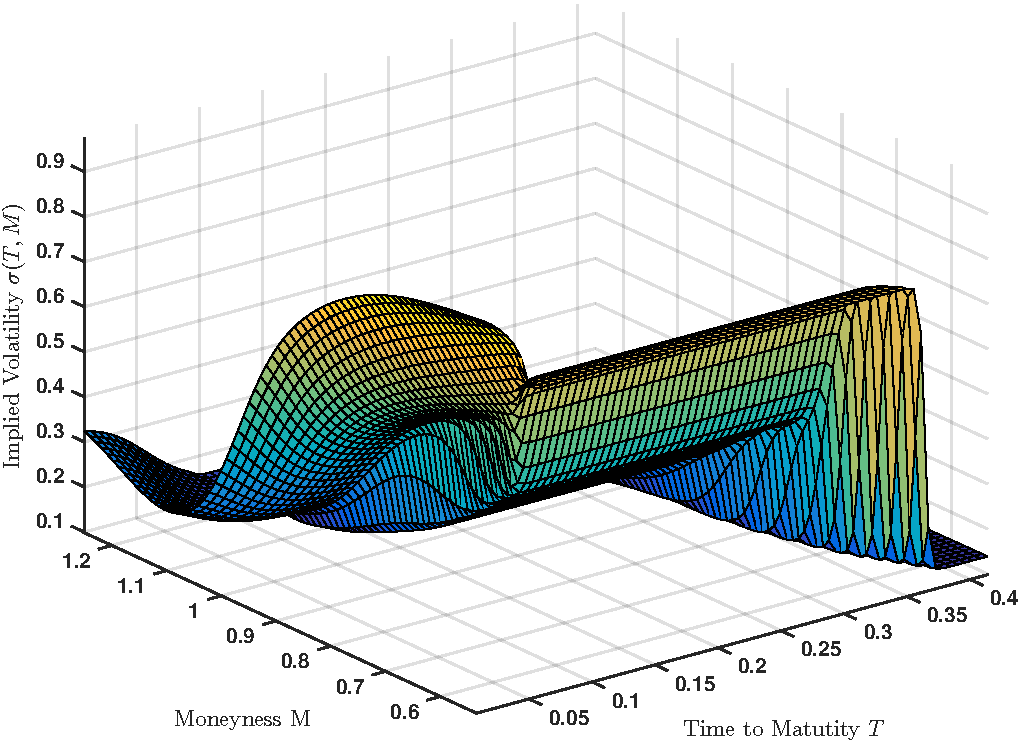
\includegraphics[width=0.80\textwidth]{../figures/blackScholesVolSurface.pdf}
  \caption{Płaszczyzna zmienności implikowanej dla indeksu $S\&P$500}
  \label{fig:volatilitySurface}
\end{figure}

Jak z niego wynika, dla opcji o bliskim terminie do wygaśnięcia opcji bardzo dobrze jest widoczny
tak zwany uśmiech zmienności (\textit{ang. volatility smile}). Stwierdzenie uśmiech 
odnosi się do faktu, że dla opcji \textit{in-the-money} oraz \textit{out-the-money}
zmienność implikowana jest o wiele wyższa niż dla opcji \textit{at-the-money} (dla opcji o krótkim
terminie do wykupu).
Jest to zarazem kolejny dowód na to, że założenie o stałości zmienności w modelu Blacka-Scholesa jest rzeczywiście niespełnione.


\section{Kalibracja}

W poprzednim podrozdziale zmienność implikowaną użytą w równaniu Blacka-Scholesa bardzo łatwo 
wyliczyć mając dane podstawowe parametry opcji. Jednak, jak opisano w czwartym rozdziale, 
kalibracja (wyznaczenie optymalnych) parametrów modelu Hestona jest skomplikowana i jest
zadaniem optymalizacyjnym.  

Kalibracji dokonamy przy pomocy dostępnej w programie \textit{Matlab} funkcji \textit{lsqnonlin}.
Jednak, aby użyć tej funkcji potrzebujemy giełdowych danych wejściowych.


Rysunek \ref{fig:calibration} przedstawia, zrzutowane na wykresie, dane, które
zostały użyte w celu kalibracji modelu (jak widać, zostały użyte ceny 
opcji i ich zmienności implikowane dla opcji o 3 różnych terminach wygaśnięcia: 
6, 13 oraz 20 dni.)

\begin{figure}
  \centering
  \includegraphics[width=0.80\textwidth]{../figures/calibrationInput.pdf}
  \caption{Dane wejściowe do funkcji kalibrującej model Hestona do danych giełdowych}
  \label{fig:calibration}
\end{figure}

W wyniku kalibracji otrzymano następujące parametry:


\begin{itemize}
  \item $V(1) = 0.0534 $
  \item $\kappa = 40.5962$
  \item $\theta = 0.0098$
  \item $\sigma = 0.0022$
  \item $\rho = 0.4031$
\end{itemize}


Mając wyznaczone zadane parametry modelu, można przejść do wyceny opcji, stosując metodę Monte Carlo.


\section{Symulacja Monte Carlo ceny europejskiej opcji kupna na indeks S\&P500}

Po znalezieniu odpowiedniej wartości nieznanych paramentów modelu Hestona, można 
przejść do symulacji Monte Carlo wyznaczającej cenę opcji o zadanych właściwościach.

W tym rozdziale wycenimy opcję kupna o następujących właściwościach:
\begin{enumerate}
  \item cena początkowa aktywa bazowego = $207.93$
  \item cena wykupu opcji = $207.93$ 
  \item zaanualizowana stopa wolna od ryzyka = $0.03$
  \item początkowa zmienność =  $0.15$
  \item czas do wygaśnięcia opcji = 412 dni
\end{enumerate}
 
Na poniższym rysunku widać wynik symulacji ceny opcji dla kilkuset losowo wybranych przebiegów.
Z definicji Monte Carlo wynika, ze poprawnym estymatorem dla wartości oczekiwanej ceny
opcji jest średnia ze wszystkich przebiegów.
Na rysunku zanaczono również poziomą linią wartość punktu startowego, tzn. wartość 
aktywa bazowego w momencie zerowym.

\begin{figure}
\centering
  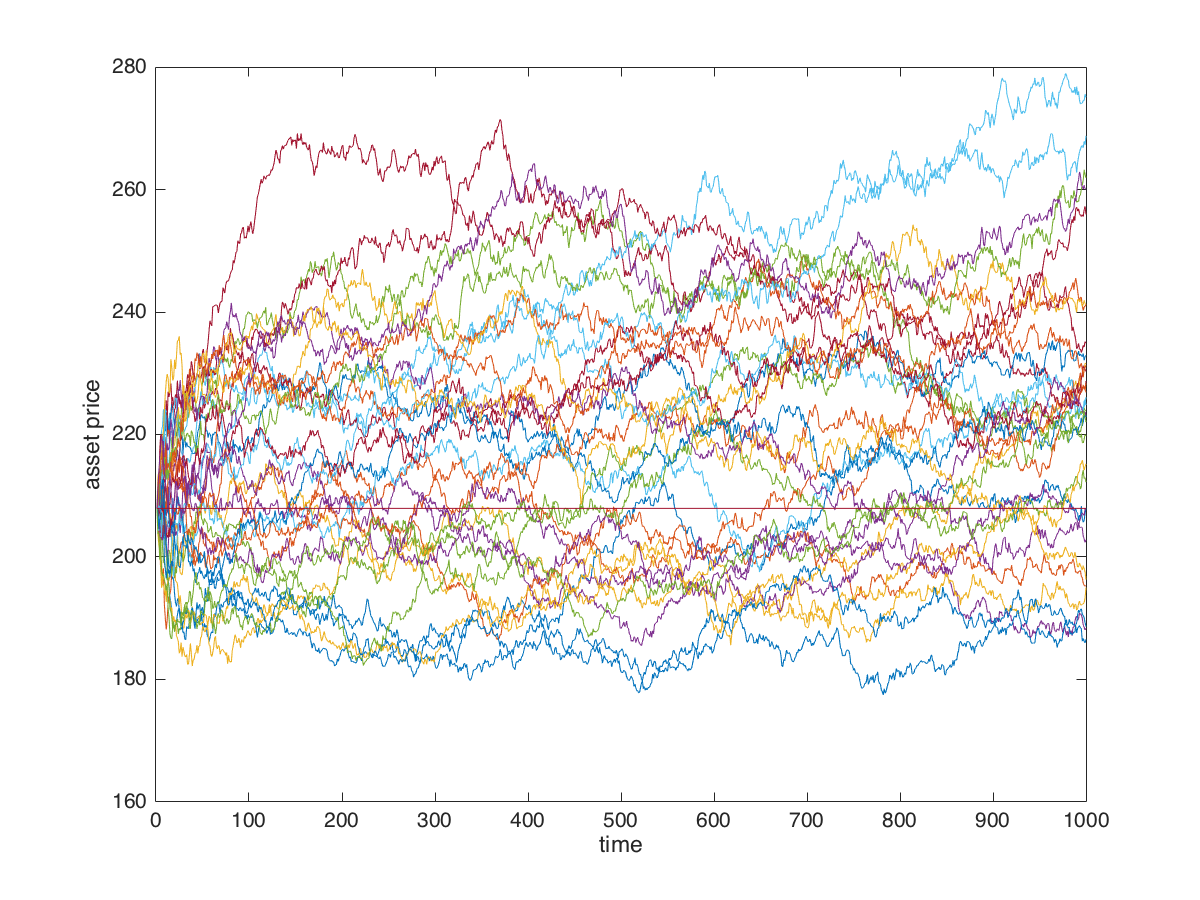
\includegraphics[width=0.80\textwidth]{../chartHeston.png}
  \caption{Trajektorie procesu cen instrumentu bazowego}
  \label{fig:hestonAssetPaths}
\end{figure}


Z wykonania symulacji dla metody Hestona wynika ze średnia cena opcji z czasem do wygaśnięcia jednego roku wynosi $13.61$ USD, 
co jest znacznie bliższe wartości wycenianej przez rynek ($13.08$ USD) w porównaniu do modelu BS. 
Przypomnijmy, że dla modelu Blacka-Scholesa, cena ta wynosiła $14.16$ USD.



\section{Współczynniki greckie dla indeksu S\&P500}


Na koniec rozdziału przedstawimy zachowanie się modelu Hestona dla jednego, wybranego wspóczynnika greckiego, 
a mianowicie dla $\Theta$.

\textit{Theta}, jako współczynnik cen opcji w zależności od upływającego czasu:
\begin{equation}
  \Theta = - \frac{\delta V}{\delta T}
\end{equation}

Rysunek \ref{fig:hestonTimeToExpiry} przedstawia zachowanie się cen opcji wraz z rosnącym czasem do 
wygaśnięcia opcji. Dla pierwszego wykresu czas do wygaśnięcia wynosi pół roku, natomiast dla ostatniego 
wynosi 6 lat. Wyraźnie widać, że trajektorie ceny instrumentu bazowego o wiele bardziej odchylają się 
na 
\begin{figure}
  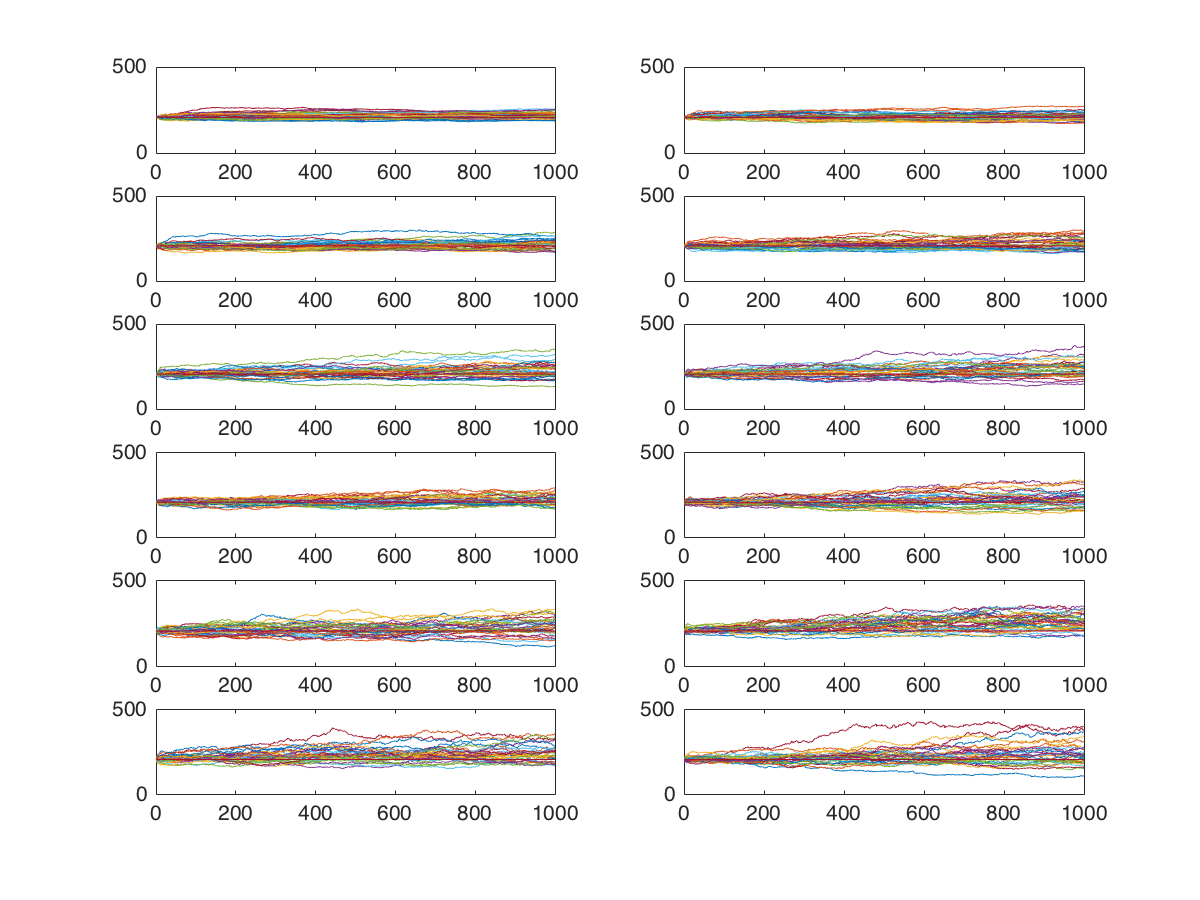
\includegraphics[width=1.00\textwidth]{../figures/hestonTimeToExpiry.pdf}
  \caption{Cena instrumentu bazowego w modelu Hestona w zależności od czasu do wygaśnięcia opcji}
  \label{fig:hestonTimeToExpiry}
\end{figure}

Jak można zauważyć, wraz z spadającym czasem do wygaśnięcia maleje potencjalny rozrzut cen aktywa bazowego w momencie wygaśnięcia opcji
Jest to zgodne z intuicją. Opcje, których cena jest zależna od zmienności instrumentu bazowego, 
w krótszym okresie czasu będą będą mniej warte od tych z dłuższym okresem do wygaśnięcia.


%===========================================================================
%                             Zakończenie
%===========================================================================
 \chapter*{Zakończenie}\label{r:ending}

Celem niniejszej pracy było porównanie modeli służących do wyceny
opcji oraz implementacja modelu Hestona, który wylicza wartość opcji biorąc
pod uwagę brak stałości w czasie zmienności, jednego z podstawowych parametrów
mającego wpływ na wycenę opcji. 

Pierwszym modelem służący do wyceny opcji jest model Blacka-Scholesa, który jest
najprostszym modelem do wyceny opcji i porównano go do efektywności modelu 
Hestona. 

Model Hestona, który jest bardziej zaawansowany koncepcyjnie, jest jednocześnie 
bardziej skomplikowany obliczeniowo. Wynika to z faktu, że ma on kilka dodatkowych
parametrów, które należy wyznaczyć na podstawie informacji z rynku. Proces wyznaczania tych 
parametrów, nazwany procesem kalibracji, jest o wiele bardziej skomplikowany w przypadku 
modelu Hestona, ponieważ tutaj jest to zadanie optymalizacyjne, natomiast w przypadku modelu
Blacka-Scholesa jest to zadanie algebraiczne.

Szczegółowo opisano również w jaki sposób należy zastosować symulację Monte Carlo do 
wygenerowania ceny opcji zgodnej z modelem Hestona. Krytycznym punktem okazał się być
proces dyskretyzacji procesu losowego. Przedstawiono dwa schematy: pierwsze naiwny, nazwany
dyskretyzacją Eulera oraz drugi bardziej dokładnego, którego wynikiem było powstanie 
algorytmu Andersena. 

Z badań empirycznych jasno wynika, że założenie o stałości zmienności w czasie nie jest 
prawdziwe dla danych rzeczywistych. Ponadto, przeprowadzono wycenę opcji na indeks 
S\&P500 dla obydwu metod: modelu Blacka-Scholesa oraz modelu Hestona. 
W porównaniu do rynkowej ceny opcji o zadanych właściwościach, obydwie metody się 
sprawdzają, jednak większą dokładność osiągnął model Hestona.


Podsumowując, można stwierdzić, że model Hestona jest o wiele bardziej zaawansowanym
narzędziem do wyceny opcji niż model Blacka-Scholesa. Uwzględniając zróżnicowanie zmienności 
w czasie sprawia, że cena opcji jest bardziej dokładna. Jednak cena jaką za to płacimy,
jest o wiele większe skomplikowanie modelu, zarówno w sferze koncepcyjnej, jak i 
implementacyjnej. Ze względu na konieczność wieloparametrowej kalibracji modelu, 
model ten jest o wiele bardziej czasochłonny obliczeniowo, niż chociażby model Blacka-Scholesa.


\appendix

\listoffigures 
\addcontentsline{toc}{chapter}{Lista rysunków} \markboth{Figures}{}
\addcontentsline{toc}{chapter}{Lista kodów źródłowych} \markboth{Listings}{}
\listoflistings
\printbibliography
\printindex 


\end{document} 